\chapter{ADT, List, Stack and Queue}

\section{Abstract Data Type (ADT)}
We use data abstraction to simplify software development since it facilitates the decomposition of the complex task of developing a software system. To put it simply, data abstraction shows only the essential details of data, while the implementation details are hidden.

For example, as will be discussed later, List, Stack, and Queue (LSQ) are forms of data abstraction, or what we call abstract data types. We can use them to retrieve or store data, but we don't know how they are actually stored or indexed.

Data encapsulation, or information hiding, is the concealing of the implementation of a data object from the outside world. Through data abstraction, we can separate the specification of a data object from its implementation.

A data type is a collection of objects and a set of operations that act on those objects. An abstract data type (ADT) is a data type organized in such a way that we can separate the specification of the object and the specification of the operations on the object. Abstract data types are simply a set of operations, and they are mathematical abstractions.

Note that abstraction is like a functional description without knowing how to use it, while implementation, on the contrary, is something that can be used and executed.

In summary, an ADT is a high-level description of how data is organized and the operations that can be performed on it. It abstracts the details of its implementation and only exposes the operations that are allowed on data structures.

\section{List}
The first abstract data type in this chapter is List.

\subsection{Definition}
When dealing with a general list of the form \(a_1, a_2, \cdots, a_n\), we say that the size of this list is \(n\). If the list is of size 0, we call it the \textbf{null list}. Except null list, we say that \(a_{i+1}\) follows/succeeds \(a_i (i < n)\) and that \(a_{i-1}\) precedes \(a_i (i > 1)\). 

The first element of the list is \(a_1\), and the last element is \(a_n\). The predecessor of \(a_1\) and the successor of \(a_n\) is not defined. 

\subsection{Operations}
A list of elements of type \(T\) is a finite sequence of elements of \(T\) together with the following operations:

- Create the list and make it empty.

- Determine whether the list is empty or not.

- Determine whether the list is full or not.

- Find the size of the list.

- Retrieve any entry from the list, provided that the list is not empty.

- Store a new entry, replacing the entry at any position in the list, provided that the list is not empty.

- Insert a new entry into the list at any position, provided that the list is not full.

- Delete any entry from the list, provided that the list is not empty.

- Clear the list to make it empty.

With these operations, we can perform various tasks on the list ADT.

\subsection{Implementation}
We can use an array to implement a list. Most of the operations follow linear time, for example, \verb|print_list|, \verb|make_null|, \verb|find|, and \verb|find_kth|. For insertion, there could be cases where the list is full, and that's why we need dynamically allocated space. For deletion, we need to find the element, perform the deletion, and reallocate space, which might require more time. Thus, we introduce the linked list.

\subsection{Linked List}
There are several types of linked lists:

\begin{center}
\begin{minipage}{0.45\textwidth}
\begin{figure}[H]
  \centering
  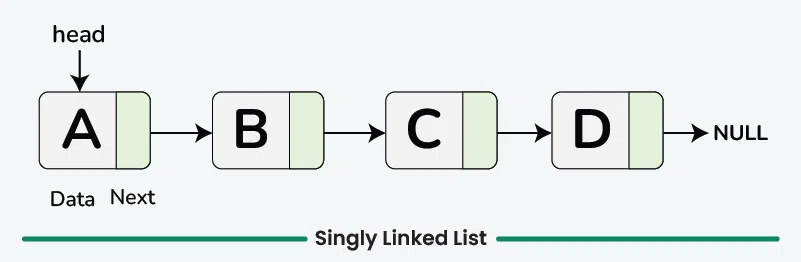
\includegraphics[width=\textwidth]{Figure/singly-linked-list.png}
  \caption{Singly Linked List}
\end{figure}
\end{minipage}\quad
\begin{minipage}{0.45\textwidth}
\begin{figure}[H]
  \centering
  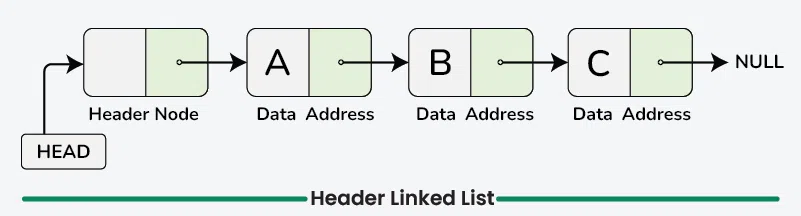
\includegraphics[width=\textwidth]{Figure/header-linked-list.png}
  \caption{Singly Linked List with Header}
\end{figure}
\end{minipage}

\begin{minipage}{0.45\textwidth}
\begin{figure}[H]
  \centering
  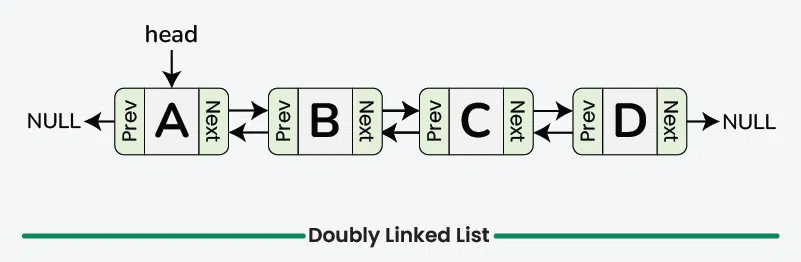
\includegraphics[width=\textwidth]{Figure/doubly-linked-list.png}
  \caption{Doubly Linked List}
\end{figure}
\end{minipage}\quad
\begin{minipage}{0.45\textwidth}
\begin{figure}[H]
  \centering
  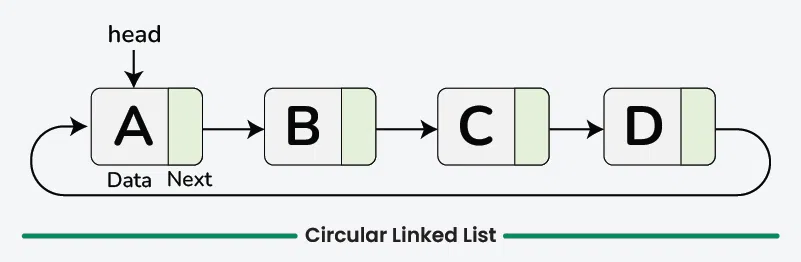
\includegraphics[width=\textwidth]{Figure/circular-linked-list.png}
  \caption{Circularly Linked List}
\end{figure}
\end{minipage}

\begin{minipage}{0.45\textwidth}
\begin{figure}[H]
  \centering
  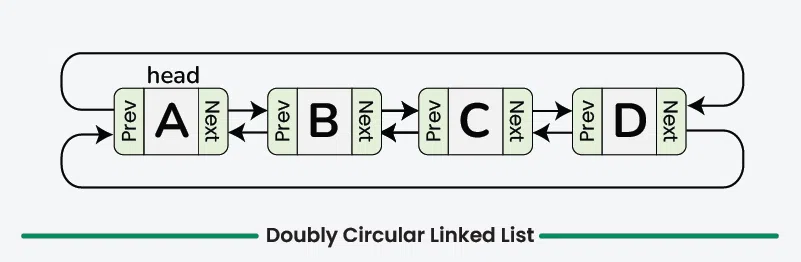
\includegraphics[width=\textwidth]{Figure/double-cir-linked-list.png}
  \caption{Circularly Doubly Linked List}
\end{figure}
\end{minipage}
\end{center}

A polynomial can be represented as
\[
  F(X) = \sum_{i = 0}^N A_{i} X^i
\]
For example, \(F(X) = 4X^3 + 2X^2 + 5X + 1\). We may want to perform operations like addition, subtraction, multiplication, and differentiation. Using an array data structure, the time complexity may be larger due to the need to store all terms, including zero coefficients. However, with a linked list, we can efficiently perform these operations by traversing the linked list and processing only the non-zero terms.

Also, note that a circular list saves space but not time. It is useful for smaller datasets. However, for a larger number of students and courses, the use of such a circular list might be a waste of space.

In summary, a list abstract data type represents an ordered collection of elements. They can be added or removed at any position in the list. It provides methods to access elements by their position.

By using different types of linked lists, we can achieve various goals. For example, we can print all the elements in reverse using a doubly linked list.

\section{Stack}
\subsection{Definition}
A stack is an ordered list in which all insertions and deletions are made at one end, called the top. It follows the Last In, First Out (LIFO) rule.

\subsection{Operations}
A stack of elements of type \(T\) is a finite sequence of elements of \(T\) along with the following operations:

- Create the stack. 

- Determine if the stack is empty or not.

- Determine if the stack is full or not.

- Determine the number of entries in the stack.

- Insert (Push) a new entry at one end of the stack, called its top, if the stack is not full.

- Retrieve the entry at the top of the stack, if the stack is not empty.

- Delete (Pop) the entry at the top of the stack, if the stack is not empty.

- Clear the stack to make it empty.

\subsection{Implementation}
We can use a doubly linked list to implement the stack, where both Push and Pop operations happen at the front of the list. We can use the Top operation to examine the element at the front of the list. In this case, the space complexity would be \(O(3n)\), and the time complexity would be \(O(c)\), where \(c\) is a constant.

Alternatively, we can use an array to implement the stack, since we only perform insertion and deletion at the top. However, we need to declare the size ahead of time and use TopOfStack as the counter to point to the top of the stack. If an array is used, the space complexity would be \(O(n)\), and the time complexity would be \(O(1)\). 

\subsection{Application}
\subsubsection{Balance Symbols}
We can use a stack to balance symbols, which is commonly used in compilers to check for syntax errors. While compiling, an empty stack is created, and an opening symbol is pushed onto the stack. Then, when a closing symbol is encountered, it is popped from the stack. There could be four types of errors:

1. Stack Overflow: Too many brackets.

2. Mismatched Symbols: The opening and closing symbols don't match.

3. Empty Stack: Attempting to pop from an empty stack.

4. Non-Empty Stack: The stack isn't empty at the end of the process.

\subsubsection{Reverse Polish Calculator}
We can also use a stack to make a Reverse Polish Calculator. There are three forms of notation: prefix, postfix, and infix. For example, if the expression is \(a \times b\), then:

1. Prefix: \(\times a b\)

2. Postfix: \(a b \times\)

3. Infix: \(a \times b\)

In Reverse Polish notation (postfix), parentheses are not needed. Using a stack, we can calculate the answer by evaluating the postfix expression. For example, when the character is a number, it is pushed onto the stack. If the character is an operator, two elements are popped from the stack, and the operation is performed on those two elements.

In summary, the stack abstract data type is a collection of elements with two main operations: push and pop. All operations happen at the top, and it follows the Last In, First Out (LIFO) approach.

\section{Queue}
\subsection{Definition}
A Queue is an ordered list in which all insertions take place at one end, the rear, while all deletions take place at the other end, the front. It follows the First In, First Out (FIFO) rule.

\subsection{Operations}
Several operations can be performed on a queue:

- Create the queue

- Determine if the queue is empty or not.

- Insert (Enqueue) a new entry at one end of the queue, called its rear, if the queue is not full.

- Delete (Dequeue) an entry at the other end of the queue, called its front, if the queue is not empty.

- Retrieve the entry at the front of the queue, if the queue is not empty.

- Clear the queue and make it empty.

\subsection{Implementation}
We can use both linear and circular arrays to implement a queue. For a linear array, we can have two indices that always increase. However, this might lead to overflow. Additionally, the array may need to be shifted forward or backward after each enqueue or dequeue operation. For a circular array, we have the following possibilities:

- Front and rear indices, with one position left vacant.

- Front and rear indices, with a Boolean variable indicating fullness or emptiness.

- Front and rear indices, with an integer variable counting entries.

- Front and rear indices taking special values to indicate emptiness.

\subsection{Application}
Queues are commonly used in various applications, such as in printer queues, airline control systems, and bank queues.

In summary, the physical model of a queue is a linear array, with the front always in the first position. All entries are moved up the array whenever the front is deleted. It follows the First In, First Out (FIFO) rule.
